% !TeX spellcheck = en_GB
% !TeX encoding = UTF-8

% COMPILE WITH:
% `latexmk`
% You need lualatex and biber (in all TeXLive distributions)
\documentclass[
numbers=noenddot,
%listof=totoc,
parskip=half-,
fontsize=12pt,
paper=a4,
oneside,
titlepage,
bibliography=totoc,
chapterprefix=false,
table
%    draft
]{scrbook}

%\usepackage[utf8]{inputenc}
%\usepackage[T1]{fontenc}
\usepackage[ngerman]{babel}
\usepackage{algorithmicx}
\usepackage{algorithm}
\usepackage{algpseudocode}
\usepackage{graphicx}
\usepackage{array}
\usepackage{amsmath}
\usepackage{pdflscape}


%pgfplots
\usepackage{pgfplots}
\pgfplotsset{width=10cm,compat=1.9} 
\usepgfplotslibrary{external}
\tikzexternalize 

% use lualatex or xelatex
%\usepackage{fontspec}
\usepackage{wrapfig}
\usepackage[onehalfspacing]{setspace}

% better language support
\usepackage{polyglossia}
\setdefaultlanguage{english}
%\setdefaultlanguage{german}

\usepackage{tocbasic}
\usepackage{booktabs}
\usepackage{multicol}
\usepackage{multirow}
\usepackage{paralist}
\usepackage[]{scrlayer-scrpage}

% better bibliography (biblatex style)
% use biber to compile
\usepackage[citestyle=alphabetic, bibstyle=alphabetic, sorting=nyt, backend=biber, language=english, backref=true, maxcitenames=2]{biblatex}

% better quotes
% use \enquote{text}
\usepackage[autostyle,english=american,german=quotes]{csquotes}
\addbibresource{bibliography.bib}

% appendix
\usepackage[titletoc]{appendix}
\usepackage[T1]{fontenc}
\usepackage{siunitx}
\usepackage{float}
\usepackage[utf8]{inputenc}
\usepackage{hyperref}
\usepackage{subfiles}
\usepackage{subfig}
%\usepackage[table]{xcolor}

% where to put all images and figures
\graphicspath{{images/}}

% Title
\title{Scratch Bug Detection Using the N-gram Language Model}

% Author
\author{Eva Gründinger}

% Date
\date{\today}

% CHOOSE ACCORDINGLY
\newcommand{\thesisType}{bachelor's thesis}
%\newcommand{\thesisType}{Masterarbeit}

\makeatletter
\let\thetitle\@title
\let\theauthor\@author
\let\thedate\@date
\makeatother

\pagestyle{scrheadings}

\begin{document}

%%%%%%%%%%%%%%%%%%%%%%%%%%%%%%%%%%%%%%%%%%%%%%%%%%%%%%%%%%%%%%%%%%%%%%%%%%%%%%%%%%%%%%%%%
\frontmatter
% CHOOSE ACCORDINGLY
% !TeX spellcheck = en_GB
% !TeX encoding = UTF-8
% !TeX root = ../thesis.tex
\begin{titlepage}
    \centering
    \begin{onehalfspace}
    
        	
\includegraphics[width=7cm]{images/uni-logo.png}\\
        	\vspace{1.0cm}
        	\large {\bfseries Chair of Software Engineering II} \\

        	\vspace{2.5cm}

            \begin{doublespace}
            	{\textsf{\Huge{\thetitle}}}
            \end{doublespace}

        	\vspace{2cm}

            \Large{Bachelor Thesis by}\\

        	\vspace{1cm}

        	{\bfseries \large{\theauthor}}

        	\vfill

        	{\large
        		\begin{tabular}[l]{cc}
        			\textsc{Advisor}\\
        			Prof.~Dr.~Gordon Fraser
        		\end{tabular}
        	}

        	\vspace{1.5cm}

        	\parbox{\linewidth}{\hrule\strut}

            \vfill

	    {\thedate}
    	
    \end{onehalfspace}
\end{titlepage}

%% !TeX spellcheck = en_GB
% !TeX encoding = UTF-8
% !TeX root = ../thesis.tex
\begin{titlepage}
    \centering
    \begin{onehalfspace}
    
        	
\includegraphics[width=7cm]{images/uni-logo.png}\\
        	\vspace{1.0cm}
        	\large {\bfseries Chair of Computer Engineering} \\

        	\vspace{2.5cm}

            \begin{doublespace}
            	{\textsf{\Huge{\thetitle}}}
            \end{doublespace}

        	\vspace{2cm}

            \Large{Master Thesis by}\\

        	\vspace{1cm}

        	{\bfseries \large{\theauthor}}

        	\vfill

        	{\large
        		\begin{tabular}[l]{cc}
        			\textsc{Advisor}\\
        			Prof.~Dr.~Stefan Katzenbeisser
        		\end{tabular}
        	}

        	\vspace{1.5cm}

        	\parbox{\linewidth}{\hrule\strut}

            \vfill

	    {\thedate}
    	
    \end{onehalfspace}
\end{titlepage}


\phantomsection
\addcontentsline{toc}{chapter}{Contents}
\tableofcontents
\newpage




% -- ABSTRACT
\newcommand{\java}{\textsc{Java}}
\newcommand{\latex}{\textsc{LaTex}}

\newtheorem{definition}{Definition}

\phantomsection
\addcontentsline{toc}{chapter}{Abstract}
% !TeX spellcheck = en_GB
% !TeX encoding = UTF-8
% !TeX root = ../thesis.tex
\chapter*{Abstract}



\newpage

% -- Acknowledgements (optional)
%% !TeX spellcheck = en_GB
% !TeX encoding = UTF-8
\chapter*{Acknowledgements}

% I would first like to thank my thesis advisor ...
\newpage

\phantomsection
\addcontentsline{toc}{chapter}{List of Figures}
% -- List of figures
\thispagestyle{empty}
\cleardoublepage
\listoffigures
\newpage

%% -- List of algorithms
%\thispagestyle{empty}
%\cleardoublepage
%%\listofalgorithms
%\newpage

\phantomsection
\addcontentsline{toc}{chapter}{List of Tables}
% -- List of tables
\thispagestyle{empty}
\cleardoublepage
\listoftables

\newpage

%%%%%%%%%%%%%%%%%%%%%%%%%%%%%%%%%%%%%%%%%%%%%%%%%%%%%%%%%%%%%%%%%%%%%%%%%%%%%%%%%%%%%%%%%
\mainmatter

% -- Chapters
% following IMRaD structure
% adjust for your liking
% !TeX spellcheck = en_GB
% !TeX encoding = UTF-8
% !TeX root = ../thesis.tex
\chapter{Introduction}\label{chap:introduction}



% !TeX spellcheck = en_GB
% !TeX encoding = UTF-8
% !TeX root = ../thesis.tex
\chapter{Background}\label{chap:background}

As this thesis merges known concepts from \scratch{} analysis and \ngram{}, we introduce the concepts our work is based on in the following sections. Section~\ref{sec:analysing-scratch} introduces \scratch{} and its functionality as a block-based programming language as well as the \scratch{} analyser \litterbox{}. Section~\ref{sec:language-models} introduces the concept of a \ngram{}. It is necessary to understand the difference between n-grams and an n-gram model and the way of using it in order to obtain valuable information about \scratch{} code.


\section{Analysing \scratch{} Programs}\label{sec:analysing-scratch}
The functionality of \scratch{} is important to understand in order to follow the main research of this thesis. The following methods and analysis are based on the programming language \scratch{} and \litterbox{} which is the basis of the evaluation and used its \AST{} as a guideline for the structure of the n-gram model. 

\subsection{The Structure of \scratch{}}\label{subsec:scratch}
\scratch{}\footnote{\url{https://en.scratch-wiki.info/wiki/Scratch}, last accessed August 19, 2020} is a block-based programming language designed for kids that was created by the \textit{Massachusetts Institute of Technology}\footnote{\url{https://web.mit.edu/}, last accessed September 06, 2020}. With over 50 million registered users and shared projects\footnote{\url{https://scratch.mit.edu/statistics/}, last accessed August 19, 2020} it is one of the most popular tools for teaching children from a young age how to develop computational thinking skills to solve problems programmatically.

The 'drag-and-drop-programming' style that \scratch{} is utilizing allows the programmer to pick from a pallet of existing blocks and build scripts by combining these code pieces like a jigsaw puzzle.
\textit{Blocks}\footnote{\url{https://en.scratch-wiki.info/wiki/Blocks}, last accessed August 19, 2020} are separated into different types that include \textit{hat, stack, reporter, boolean,} and \textit{cap}. Each data type has a specific shape that indicates their intended usage in order to avoid errors in the syntax of the code. In contrast to text-based programming languages, the \textit{blocks} help children to memorize the commands and avoid structure errors that otherwise would very likely occur in the beginning. 

After combining different \textit{blocks}, \textit{scripts}\footnote{\url{https://en.scratch-wiki.info/wiki/Script}, last accessed August 19, 2020} are created which resemble code methods in \java{}. \textit{Scripts} are found in the code of the actors that perform the actions, called \textit{sprites}\footnote{\url{https://en.scratch-wiki.info/wiki/Sprite}, last accessed August 19, 2020} as well as the \textit{stage}\footnote{\url{https://en.scratch-wiki.info/wiki/Stage}, last accessed August 19, 2020} which visualises the background of the created program. 

Figure~\ref{fig:scratchblocks} shows the typical structure of a \scratch{} \textit{script} that uses most of the before mentioned data types. Starting the \textit{script} with a \textit{hat} and ending with a \textit{cap} block, there are also 10 different categories that each block is assigned to: \textit{Motion, Looks, Sound, Event, Control, Sensing, Operators, Variables, List,} and \textit{My Blocks}. 

\begin{figure}[hbtp]
    \centering
    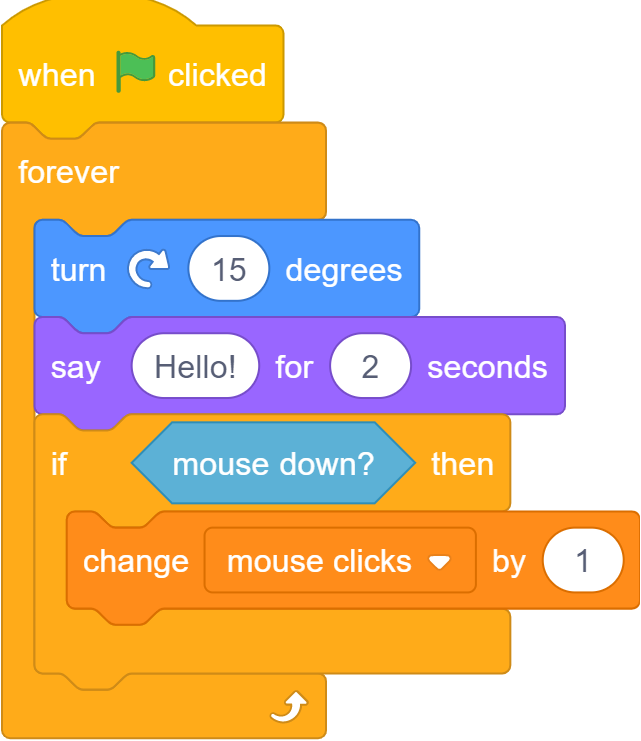
\includegraphics[scale=0.4]{scratchblocks.png}
    \caption[A representative \scratch\ script]{\label{fig:scratchblocks} A representative script in \scratch{}.}
\end{figure}

For instance, Figure~\ref{fig:script} of an example \scratch{} project\footnote{\url{https://scratch.mit.edu/projects/308718195/}, last accessed August 20, 2020} shows a \textit{script} that controls the picture of Jungkook, a member of the band BTS, which is shown in Figure~\ref{fig:sprite}. Once the user clicks on the picture of Jungkook, the 'click' event of the \textit{script} is executed and the text "Saranghae <3" is shown for 2 seconds.

\begin{figure}[hbtp]
    \centering
    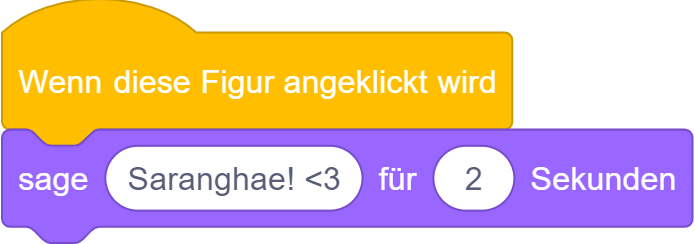
\includegraphics[scale=0.4]{jungkook_script.png}
    \caption[Script code controlling a sprite]{\label{fig:script} A \scratch\ script controlling a corresponding sprite}
\end{figure}

\begin{figure}[hbtp]%
    \centering
    \subfloat[Sprite in front of a background]{{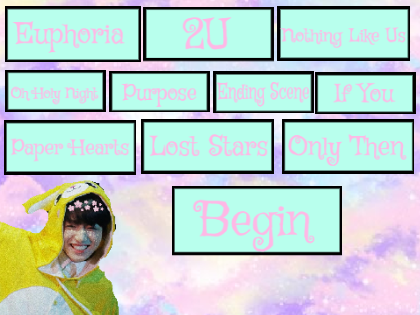
\includegraphics[width=7cm]{jungkook_stage.png} }}%
    \qquad
    \subfloat[Sprite responding to an event]{{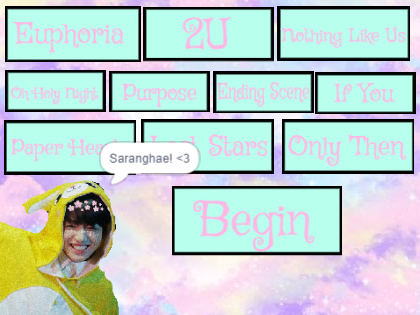
\includegraphics[width=7cm]{jungkook_stage_action.png} }}%
    \caption[A sprite's reaction after an executed event]{\label{fig:sprite}A \scratch\ stage and sprite that respond to events}%
\end{figure}

\subsection{The Static \scratch{} Code Analyser \litterbox{}}\label{subsec:litterbox}
\litterbox{}\footnote{\url{https://gitlab.infosun.fim.uni-passau.de/se2/litterbox}, last accessed August 19, 2020} is a static code analysis tool for detecting bugs in \scratch{} projects where \scratch{} code is saved as a JSON file and downloaded, for example, using the \scratch{} REST API\footnote{\url{https://projects.scratch.mit.edu}, last accessed August 20, 2020}. \litterbox{} then creates an abstract syntax tree (\AST{}) for a \scratch{} project. The occurrence of bugs in code is mostly the consequence of recurring bad code writing habits. With the help of \litterbox{} these bug patterns and code smells can be filtered and analysed in order to correct the found bugs and avoid similar mistakes in the future. \litterbox{} is developed at the Chair of Software Engineering II and the Didactics of Informatics of the University of Passau and is the foundation for the analysis of \scratch{} programs with n-gram models in this bachelor's thesis. 


\section{N-gram Language Model}\label{sec:language-models}
Statistical language models, in its essence, are the type of models that assign probabilities to sequences of words. The \ngram{} is the simplest model that assigns probabilities to sentences and sequences of words. You can think of an n-gram as the sequence of N words. A 2-gram or bigram is a two-word sequence of words like 'please read', 'read very', or 'very carefully', and a 3-gram or trigram is a three-word sequence of words like 'please read very', or 'read very carefully'. 

\subsection{Probability Calculation of N-grams}\label{subsec:ngram}
\ngram{s} usually consist of sentences \textit{s} of words \textit{w} that are all based on a specific dictionary \textit{D}. Using \hyperref[def:markov_chain]{\textit{Markov chains}} the language model calculates a probabilistic distribution of all possible sequences that can occur in the language based on \textit{D}.

\begin{definition}[Markov chain]\label{def:markov_chain}
    %
    ``A usually discrete stochastic process (such as a random walk) in which the probabilities of occurrence of various future states depend only on the present state of the system or on the immediately preceding state and not on the path by which the present state was achieved.''~\cite{markov_chain}
    %
\end{definition} 

The probability of \textit{s} is then calculated by partitioning it into its individual words \textit{w}. But the probability of \textit{w} is only dependent on the n - 1 previous words. Given a sentence \( s = w_1w_2w_3\cdots w_m \) the probability is estimated with the Formula~\ref{eq:ngram-prob} where \(h_i = w_{1-n}\cdots w_i \) is the history sequence for the conditional probability of \(w_i\):

\begin{equation} \label{eq:ngram-prob}
P(s) ={} \displaystyle\prod_{i=1}^{m} P(w_i|h_{i-1})
\end{equation}

For instance in the case of a 3-gram, each word is dependent on the probability of the last \(n - 1 = 3 - 1 = 2 \) words. Therefore the probability of the sentence s = 'Would you like to go outside?' can be estimated with the Formula~\ref{eq:trigram-prob}:

\begin{equation}\label{eq:trigram-prob}
\begin{aligned}
P(s) ={} & P(Would)\cdot P(you|Would)\cdot P(like|Would\ you) \\ 
		 & \cdot P(to|you\ like)\cdot P(go|like\ to)\cdot P(outside|to\ go)
\end{aligned}
\end{equation} 
  
\subsection{N-gram Model Configuration}\label{subsec:configuration}
There are five key factors that affect the number of bugs that a language model can find. These are the important \textit{configuration parameters} that need to be set in order to achieve optimal results:  

\begin{definition}[Gram Size]\label{def:gram_size}
    %
    ``The size of an n-gram model. Different gram sizes enable the model to use different internal probabilities to calculate the probabilities of \hyperref[def:token]{\textit{token}} sequences.''~\cite{bugram}
    %
\end{definition}

The \hyperref[def:gram_size]{\textit{gram size}} n is an essential part of building an \ngram{} and calculating the probabilities of a token sequence by utilizing n - 1 predecessors. Existing studies found that 3 to 6-gram models gave the best results, although the optimal \hyperref[def:gram_size]{\textit{gram size}} for bug detection is still unknown. 

\begin{definition}[Sequence Length]\label{def:sequence_length}
    %
    ``The length of token sequences to be considered when building n-gram models and detecting bugs. Different sequence lengths enable the model to capture different program scenarios and further affect the performance of the bug detection.''~\cite{bugram}
    %
\end{definition}

The \hyperref[def:sequence_length]{\textit{length}} of analysed sequences of a project is essential to get a detailed analysis of the project's structure. The number of code blocks and scripts in a \scratch{} project can vary from 1 to a few hundred. By partitioning a program into smaller parts, more bugs can be obtained.

\begin{definition}[Reporting Size]\label{def:reporting_size}
    %
    ``The number of sequences, in the bottom of the ranked list, which will be reported as bugs. An appropriate number may reduce the amount of false positives.''~\cite{bugram}
    %
\end{definition}

In contrast to the usual rule-based bug finding techniques which use a probability threshold to distinguish potential bugs from normal sequences, the \ngram{} detects token sequences of low absolute probabilities. A larger number of bugs that get reported from the found list will definitely lead to a bigger size of found bugs but also means a higher risk of reporting sequences that are normal occurrences.

\begin{definition}[Minimum Token Occurrence]\label{def:minimum_token_occurrence}
    %
    ``The minimum number of times a token must occur in the code to be included in an n-gram model. An appropriate value helps to filter out \hyperref[def:token]{token} sequences that use unusual/special methods, thus have low probabilities but are not bugs.''~\cite{bugram}
    %
\end{definition}

Taking out tokens in a project that are not frequently used by using a \hyperref[def:minimum_token_occurrence]{\textit{minimum token occurrence}} is common practice for natural language processing (NLP) techniques. It reduces the chances of falsely reporting uncommon token sequences that are not bugs but very rarely used. 

\begin{definition}[Probability Threshold]\label{def:probability_threshold}
    %
    ``If a \hyperref[def:token]{\textit{token}} sequence does not reach this probability threshold, it can be considered a bug or unusual occurrence.''
    %
\end{definition}

After the analysis of a project, a number of sequences with the least calculated probabilities are getting reported as bugs. But in order to minimize the number of false positives in the bug set, it is common practice to determine a \hyperref[def:probability_threshold]{\textit{probability threshold}} that differentiates a bug from a rare occurrence of a sequence. 
% !TeX spellcheck = en_GB
% !TeX encoding = UTF-8
% !TeX root = ../thesis.tex
\chapter{Methods}\label{chap:methods}


% !TeX spellcheck = en_GB
% !TeX encoding = UTF-8
% !TeX root = ../thesis.tex

\newcommand{\numlarge}{75,277}
\newcommand{\monthstart}{December 2019}
\newcommand{\monthend}{January 2020}
\newcommand{\parsingexcp}{114}
\newcommand{\successfullyanalysed}{74,914}
\newcommand{\calculatedngrams}{138,298}
\newcommand{\creationtime}{17 days}

\chapter{Evaluation}\label{chap:evaluation}

The main research points for this bachelor's thesis are answers to the following questions:
\begin{itemize}
\item[\textbf{RQ1}] How effective are \ngram{s} for bug detection in comparison to \litterbox{}?
\item[\textbf{RQ2}] What kinds of violations were detected by the \ngram{}?
\item[\textbf{RQ3}] Does the \ngram\ work in the case of open task solutions?
\item[\textbf{RQ4}] Efficiency of general \ngram\ vs project-specific model?
\end{itemize}

In the following analysis, parameters for the \ngram\ configuration were determined, like it is described in Subsection~\ref{subsec:configurations}. The \hyperref[def:gram_size]{\textit{gram size}} of 3 is adopted from the \bugram{}~\cite{bugram} paper. For the \hyperref[def:sequence_length]{\textit{sequence length}} we got the best results with the lengths 2 and 3. Furthermore, the \hyperref[def:probability_threshold]{\textit{probability threshold}} was manually estimated for each \ngram{}. The value that distinguished the most true bugs from false positives was chosen.


\section{Data Sets and Models}\label{sec:dataset}
RQ1, RQ2 and RQ3 are all answered by using project-specific models (Subsection~\ref{subsec:bugset}) and analysing representative projects of different pupil tasks. In RQ4 the general model (Subsection~\ref{subsec:trainingset}) which is based on a bigger data set is compared to the reports of the project-specific models.

\subsection{Big Data Set}\label{subsec:trainingset}
In order to have a sufficient number of sequences to calculate a probability distribution from and as comparison to the smaller project-specific models, we decided to build an \ngram{} on a large data set with its statistics shown in Table~\ref{tab:general-model}. The dataset consists of \numlarge\ \scratch\ projects. From \monthstart\ to \monthend\ we downloaded the most recent projects with the \scratch\ REST API\footnote{\url{https://github.com/LLK/scratch-rest-api/wiki}, last accessed May 8, 2020}. We did exclude remixes from the data set. \litterbox\ could not parse \parsingexcp\ projects, thus the \ngram\ was created of \successfullyanalysed\ projects without any exceptions and consists of \calculatedngrams\ calculated n-grams. The creation of the model took \creationtime\ and was conducted on machines equipped with Intel Xeon E5-2650 v2 @ 2.60 GHz CPUs with 256 GiB of RAM.

\begin{table}[hbtp]
    \centering
    \caption[General model statistics]{\label{tab:general-model}General model statistics.}
    \begin{tabular}{lrrr}
        \toprule
        File & Size & \#Projects & \#Ngrams\\
        \midrule
        \texttt{model.csv} & 7,865 KB & 74,914 & 138,298 \\
        \bottomrule
    \end{tabular}
\end{table}

\subsection{Pupils' Projects}\label{subsec:bugset}
The creation of the project-specific models as well as bug detection with the pupils' projects was done in a few seconds for every set of solutions and did not throw any exceptions. All experiments with the small data sets were conducted on a Swift SF314-57 with an Intel i5 core and 8 GB RAM.

\paragraph{Project-specific Models.}
The project-specific models with further statistics shown in Table~\ref{tab:specific-model} are build on a set of correct as well as defective solutions of five small coding tasks for students. Based on the task the pupils had to implement, we call these sets \textit{Monkey}, \textit{Elephant}, \textit{Cat}, \textit{Horse} and \textit{Fruit Catching} task. We used solutions of pupils which originate in primary programming education~\cite{katharina} for the \textit{Monkey}, \textit{Elephant}, \textit{Cat} and {Horse} tasks. For the \textit{Fruit Catching} task we used the same data set as Stahlbauer et al. in their work about testing \scratch\ programs automatically~\cite{whisker}. In addition, a set of open task solutions that pupils could experiment with was used for Section~\ref{sec:open}. 

\begin{table}[hbtp]
    \centering
    \caption[Project-specific model statistics]{\label{tab:specific-model}Project-specific model statistics.}
    \begin{tabular}{lrrrr}
        \toprule
        Task & File & Size & \#Projects & \#Ngrams \\
        \midrule
        Fruit Catching & \texttt{fruit\_model.csv} & 226 KB & 42 & 3,257  \\
        Monkey & \texttt{monkey\_model.csv} & 33 KB & 120 & 477 \\
        Elephant & \texttt{elephant\_mode.csv} & 39 KB & 130 & 559 \\
        Cat & \texttt{cat\_model.csv} & 49 KB & 129 & 715 \\
        Horse & \texttt{horse\_model.csv} & 30 KB & 73 & 440 \\
        Open & \texttt{open\_model.csv} & 101 KB & 295 & 1,897 \\
        \bottomrule
    \end{tabular}
\end{table}

\paragraph{Bug Detection.}
For bug detection we chose one representative project of each task which are listed in Table~\ref{tab:buggy-projects} and analysed them with \litterbox\ as well as the created n-gram models for the research questions. 

\begin{table}[hbtp]
    \centering
    \caption[Representative projects of each task for bug detection]{\label{tab:buggy-projects}Representative projects for each task used for bug detection.}
    \begin{tabular}{lrrrr}
        \toprule
        Task & Project & Size & \#Sprites & \#Blocks\\
        \midrule
        Fruit Catching & \texttt{K7\_S02.sb3} & 176 KB & 3.0 & 81.0\\
        Monkey & \texttt{ID\_065\_Aufgabe-Affenjagd.sb3} & 181 KB & 3.0 & 18.0 \\
        Elephant & \texttt{ID\_118\_Aufgabe-Elefant.sb3} & 456 KB & 4.0 & 23.0 \\
        Cat & \texttt{ID\_005\_Aufgabe-Katze.sb3} & 86 KB & 2.0 & 14.0 \\
        Horse & \texttt{ID\_080\_Aufgabe-Pferd.sb3} & 6 KB & 1.0 & 14.0 \\
        Open & \texttt{m043.sb3} & 304 KB & 3.0 & 26.0 \\ 
        Open & \texttt{m052-Zauberei.sb3} & 869 KB & 7.0 & 18.0 \\
        Open & \texttt{m067-Apfelsuche.sb3} & 330 KB & 3.0 & 31.0 \\
        Open & \texttt{m074-Sternenjaeger.sb3} & 58 KB & 12.0 &  65.0 \\
        Open & \texttt{m091 2.sb3} & 53 KB & 7.0 & 70.0 \\
        Open & \texttt{w002-Weltraumangriff.sb3} & 703 KB & 7.0 & 57.0 \\
        \bottomrule
    \end{tabular}
\end{table}

\paragraph{Project-specific Model Reports.}
The created boxplot in Figure~\ref{fig:boxplot1} visualises a distribution of the reported sequences for all pupil projects. We can see that each task has a different number of sequences that were detected as potential bugs with the \textit{Fruit Catching} task being the one with the most reported sequences. The huge difference between the \textit{Fruit Catching} task and the rest of the tasks is probably related to its big block counts in the projects which ultimately leads to a higher number of reported sequences.

\begin{figure}[hbtp]
    \centering
    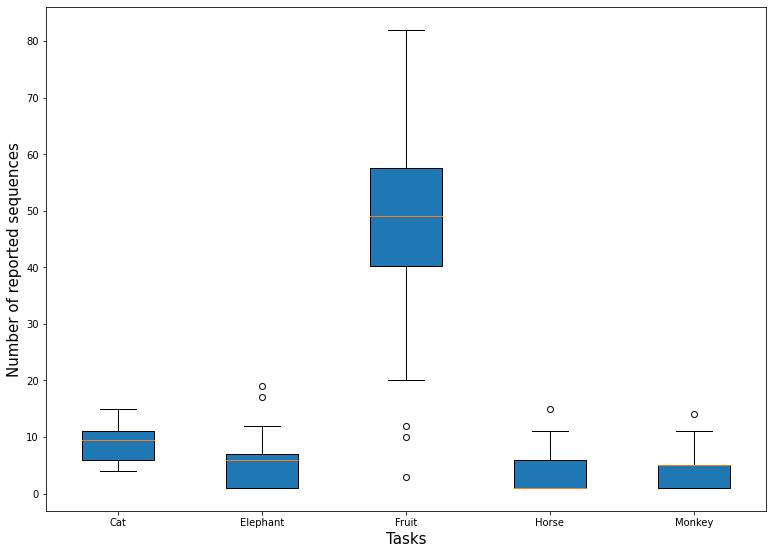
\includegraphics[scale=0.4]{boxplot_sequences.png}
    \caption[Boxplot for distribution of reported sequences]{\label{fig:boxplot1}Boxplot for distribution of reported sequences.}
\end{figure}

As a comparison to Figure~\ref{fig:boxplot1}, Figure~\ref{fig:boxplot2} shows a distribution of all reported sequences that have an occurrence probability below the estimated \hyperref[def:probability_threshold]{\textit{probability thresholds}} and therefore are more likely to be true bugs or unusual use cases than false positives.

\begin{figure}[hbtp]
    \centering
    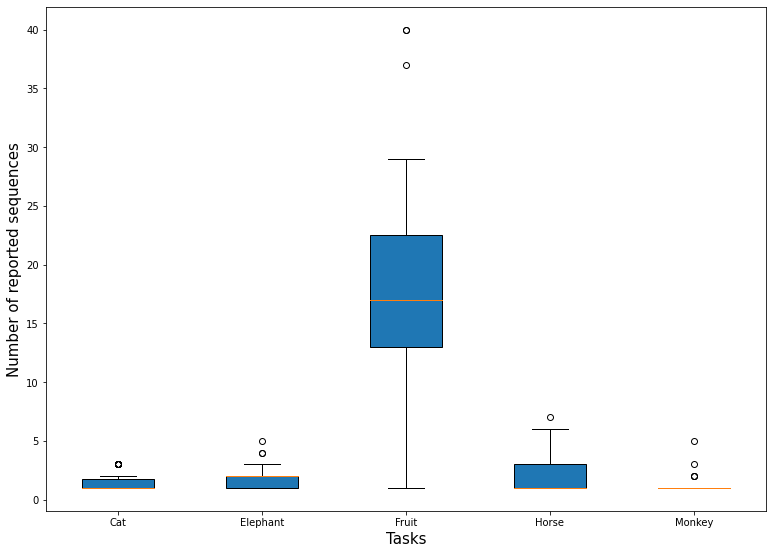
\includegraphics[scale=0.4]{boxplot_threshold.png}
    \caption[Boxplot for distribution of reported sequences with probability thresholds]{\label{fig:boxplot2}Boxplot for distribution of reported sequences with probability thresholds.}
\end{figure}

\begin{figure}[hbtp]
    \centering
    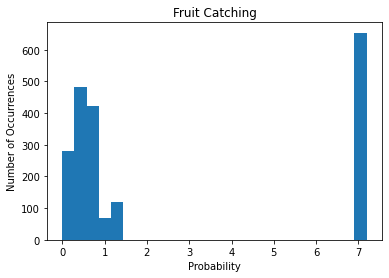
\includegraphics[scale=0.5]{fruit_his.png}
    \caption[Histogram for probability distribution of \textit{Fruit Catching} task]{\label{fig:fruit_his}Histogram of \textit{Fruit Catching} task with a \hyperref[def:probability_threshold]{\textit{probability threshold}} of 0.6\%.}
\end{figure}

\begin{figure}[hbtp]%
    \centering
    \subfloat{{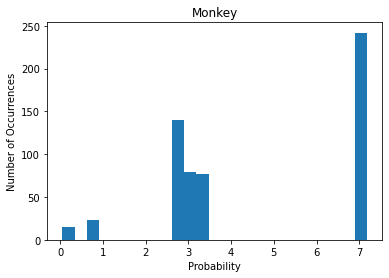
\includegraphics[width=7cm]{monkey_his.png} }}%
    \qquad
    \subfloat{{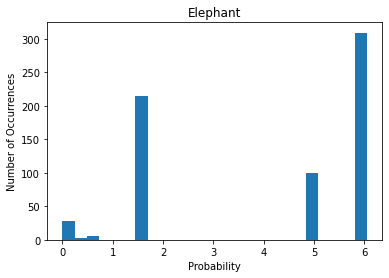
\includegraphics[width=7cm]{elephant_his.png} }}%
    \caption[Histograms of \textit{Monkey} and \textit{Elephant} tasks]{\label{fig:his1}Histograms of \textit{Monkey} and \textit{Elephant} tasks with a  \hyperref[def:probability_threshold]{\textit{probability threshold}} of 1.6\%.}%
\end{figure}

\begin{figure}[hbtp]%
    \centering
    \subfloat{{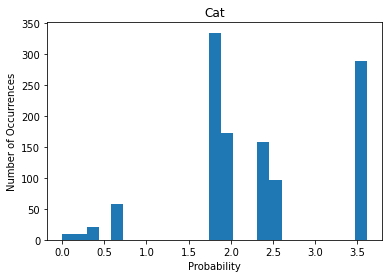
\includegraphics[width=7cm]{cat_his.png} }}%
    \qquad
    \subfloat{{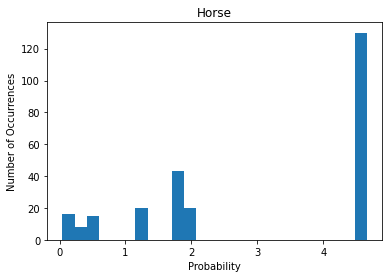
\includegraphics[width=7cm]{horse_his.png} }}%
    \caption[Histograms of \textit{Cat} and \textit{Horse} tasks]{\label{fig:his2}Histograms of \textit{Cat} and \textit{Horse} tasks with a  \hyperref[def:probability_threshold]{\textit{probability threshold}} of 1.6\%.}%
\end{figure}

The histograms of Figures~\ref{fig:fruit_his}, ~\ref{fig:his1} and ~\ref{fig:his2} show the probability distributions of the reported sequences for each task. The estimated \hyperref[def:probability_threshold]{\textit{probability thresholds}} can be seen in the figures as separations of low probability sequences to usual occurrences. A manual examination confirmed that below the chosen  \hyperref[def:probability_threshold]{\textit{probability thresholds}} the probability of false positives is very small.


\section{RQ1: Comparison to Litterbox}\label{sec:litterbox}
After setting the \hyperref[def:gram_size]{\textit{gram size}} to 3 and \hyperref[def:sequence_length]{\textit{sequence lengths}} to 2 for the first analysis and 3 for the second bug detection analysis, project-specific models for each pupil task from Table~\ref{tab:specific-model} are used for a comparison between \litterbox~\cite{scratch_bugpatterns} and the \ngram{} approach of \bugram~\cite{bugram}. The same projects from Table~\ref{tab:buggy-projects} are analysed by \litterbox{} and the \ngram{} to test how many sequences are reported after knowing the failed tests of each project through \whisker~\cite{whisker}. The \hyperref[def:reporting_size]{\textit{reporting size}} is unlimited in this case. Table~\ref{tab:litterbox} shows the number of reported smells or sequences of each method. 

\begin{table}[hbtp]
    \centering
    \caption[The number of reported bugs found by \litterbox{} and n-gram model]{\label{tab:litterbox}The number of reported bugs found by \litterbox{} and n-gram model.}
    \begin{tabular}{lrrr}
        \toprule
        Task & \#FailedTests & \#LitterboxSmells & \#NgramSequences \\
        \midrule
        Fruit Catching & - & 113 & 42 \\
        Monkey & 0 & 2 & 8 \\
        Elephant & 0 & 1 & 5 \\
        Cat & 0 & 0 & 6 \\
        Horse & 1 & 0 & 8 \\
        \bottomrule
    \end{tabular}
\end{table}

The analysis shows that even though in some cases \litterbox\ did not find smells and \whisker\ tests all passed, the \ngram\ reported sequences that pointed out potential bugs or unusual use cases. This shows that the \ngram\ has a different range of violations it can detect in \scratch\ projects.


\section{RQ2: Violation Classification}\label{sec:violations}
The analysis procedure is continued by analysing specifically the bugs that are reported by the \ngram{}. For each task one project is manually analysed to estimate the rate of false positives. The \hyperref[def:probability_threshold]{probability threshold} varies from the size of the model. Table~\ref{tab:buggy-projects} shows the projects that were chosen for assessment as well as their further information. After all by the \ngram{} detected potential bugs were collected in the candidate bug set, the defective code is manually classified into the following categories: \textit{True Bugs}, \textit{Unusual Use Cases} or \textit{False Positives}. Table~\ref{tab:violations} displays the numbers for each category.

\begin{table}[hbtp]
    \centering
    \caption[The categorization of all reported bugs]{\label{tab:violations}The categorization of all reported bugs.}
    \begin{tabular}{lrrrrr}
        \toprule
        Task & \parbox[t]{2.2cm}{Probability\\Threshold} & \#Reported & \#True & \#UnusualUse & \#FalsePositive \\
        \midrule
        Fruit Catching & 0.6\% & 23 & 15 & 3 & 5 \\
        Monkey & 1.6\% & 3 & 2 & 1 & 0 \\
        Elephant & 1.6\% & 1 & 0 & 1 & 0 \\
        Cat & 1.6\% & 1 & 0 & 1 & 0 \\
        Horse & 1.6\% & 4 & 3 & 0 & 1 \\
        \bottomrule
    \end{tabular}
\end{table}

If a sequence is an unusual use case, it will not be detected by \litterbox\ because it is not a code smell. Most of the time an unusual use is a consequence of an extension of the original task and therefore not part of the usual used sequences that are needed for a project to pass the test. 

\begin{table}[hbtp]
    \centering
    \caption[An excerpt of the report for the \textit{Fruit Catching} task]{\label{tab:report}An excerpt of the report for the \textit{Fruit Catching} task.}
\begin{tabular}{lrrr}
        \toprule
        Actor & Position & Sequence & Probability\\
        \midrule
        Bowl & Script@1608d14c & RepeatTimesStmt, NumberLiteral & 0.06948304613674264 \\
	   Apple & Script@1ff8da & Never, UntilStmt & 0.44469149527515284 \\
	   Apple & Script@3a4e11a & IfElseStmt, UnspecifiedBoolExpr & 0.023346303501945526 \\
	   Apple & Script@e3e2beb8 & ChangeYBy, NumberLiteral & 0.39355197331851033 \\
        \bottomrule
    \end{tabular}
\end{table}

\begin{figure}[hbtp]%
    \centering
    \subfloat[Example \scratch\ code.]{{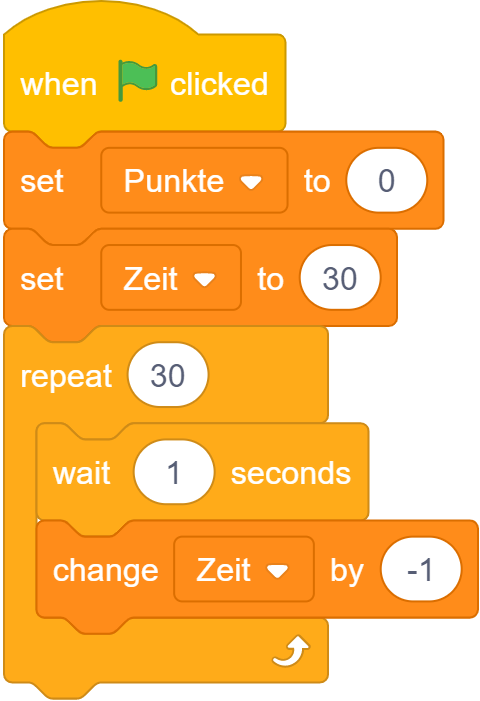
\includegraphics[width=5cm]{unusualUse.png} }}%
    \qquad
    \subfloat[RepeatTimesStmt, NumberLiteral]{{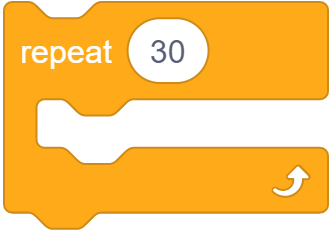
\includegraphics[width=5cm]{reportedUnusualUse.png} }}%
    \caption[Example \textit{script} for detected unusual use case in \scratch\ code]{\label{fig:unusualUse}Example \textit{script} for detected unusual use case in \scratch\ code.}%
\end{figure}

Figure~\ref{fig:unusualUse} from the project \texttt{K7\_S02.sb3} shows an example for an unusual use case with the sequence [RepeatTimesStmt, NumberLiteral] that was reported with a probability of 0.07\%, according to the report excerpt in Table~\ref{tab:report}. This means that in the solutions of the \textit{Fruit Catching} task, the usage of a [RepeatTimesStmt] block was very limited and therefore it is despite its low probability not a bug.  

\begin{figure}[H]
    \centering
    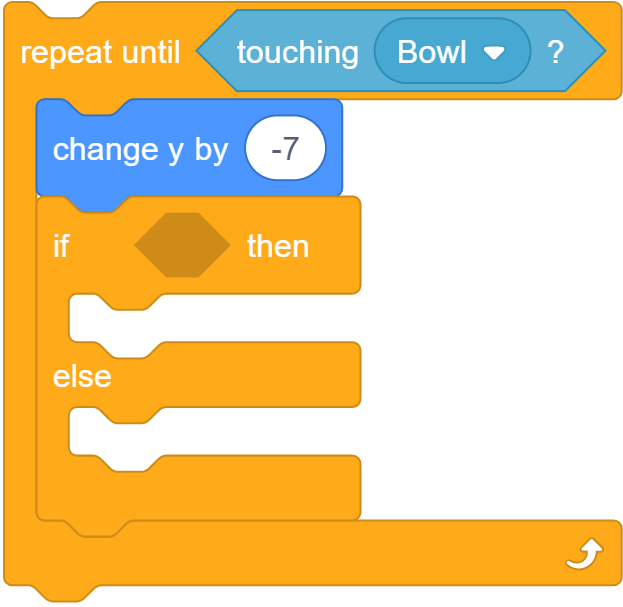
\includegraphics[scale=0.4]{trueBug.png}
    \caption[Example for detected bug and false positive in \textit{Fruit Catching} project]{\label{fig:trueBug}Example for detected bug and false positive in \textit{Fruit Catching} project.}
\end{figure}

Another example would be the \textit{script} in Figure~\ref{fig:trueBug} where everyone can see at first glance that there is a bug that is caused by missing \textit{blocks}. The reported sequences, that are also shown in Table~\ref{tab:report}, are [Never, UntilStmt] with 0.44\%, [IfElseStmt, UnspecifiedBoolExpr] with a probability of 0.02\% and [ChangeYBy, NumberLiteral] with 0.39\% although the last sequence is classified as a false positive. 

When we compare the code smells that \litterbox\ is able to find with the bugs that can be detected by the \ngram{}, then we see that the \ngram\ is not able to detect long scripts or unused variables in the \scratch\ code. But the \ngram\ is capable of finding dead code, empty scripts as well as empty bodies in if-else statements. 
 

\section{RQ3: Open Solutions}\label{sec:open}
For a wider perspective on the usage of the \ngram\ approach to bug detection we selected a set of pupils' solutions where the children could try out all the things they had newly learned. This means that there is no unique solution for these tasks, just open interpretations of simple projects. Therefore, there is no method to determine if a reported sequence is an unusual use case. The project-specific model, we created out of the solutions, reported the following bugs displayed in Table~\ref{tab:open} for a set of example projects of the data set. In this analysis the \hyperref[def:probability_threshold]{\textit{probability threshold}} is set to 0.5\% for the model. 

\begin{table}[hbtp]
    \centering
    \caption[Open projects report]{\label{tab:open}Reported bugs of open projects.}
    \begin{tabular}{lrrr}
        \toprule
        Task & \#Reported & \#TrueBug & \#FalsePositive \\
        \midrule
        \texttt{m043.sb3} & 4 & 3 & 1 \\   
        \texttt{m052-Zauberei.sb3} & 2 & 1 & 1 \\ 
        \texttt{m067-Apfelsuche.sb3} & 1 & 0 & 1 \\
        \texttt{m074-Sternenjaeger.sb3} & 1 & 0 & 1 \\
        \texttt{m091 2.sb3} & 4 & 0 & 4 \\
        \texttt{w002-Weltraumangriff.sb3} & 2 & 2 & 0 \\            
        \bottomrule
    \end{tabular}
\end{table}

The frequent occurrence of false positives could be a consequence of the missing unusual use case categorisation. A lot of sequences just were not used as often by the novice programmers and when they appear one time their probability is consequently pretty low. 

\begin{table}[hbtp]
    \centering
    \caption[An excerpt of the report for the \textit{Zauberei} task]{\label{tab:report2}An excerpt of the report for the \textit{Zauberei} task.}
\begin{tabular}{lrrr}
        \toprule
        Actor & Position & Sequence & Probability\\
        \midrule
    	   Rokkduck & Script@497b81c5 & PlaySoundUntilDone, Never & 0.16643473084111865 \\
        Rokkduck & Script@497b81c5 & RepeatTimesStmt, NumberLiteral & 0.3615592433603648 \\
        \bottomrule
    \end{tabular}
\end{table}

\begin{figure}[hbtp]
    \centering
    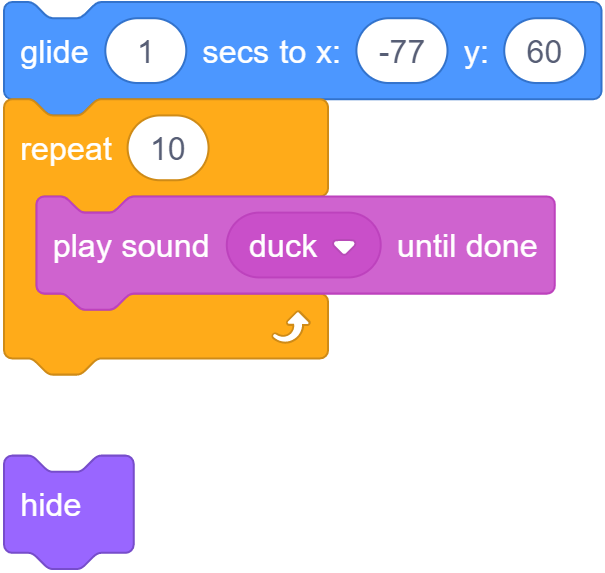
\includegraphics[scale=0.4]{openBugs.png}
    \caption[Example for detected bug and false positive in open project]{\label{fig:openBugs}Example for detected bug and false positive in open project.}
\end{figure}

The \scratch\ \textit{script} in Figure~\ref{fig:openBugs} is a part of the \texttt{m052-Zauberei.sb3} code and contains an example for a bug as well as false positive that are shown in the report excerpt in Table~\ref{tab:report2}. The sequence [PlaySoundUntilDone, Never] with a probability of 0.17\% is a bug because it hints at the [Hide] block that can never be executed because of a missing \textit{hat} block. Furthermore, the sequence [RepeatTimesStmt, NumberLiteral] with 0.36\% is falsely reported because it is not a programming mistake. If there was a reference solution of the \textit{Zauberei} task, then it could also be an unusual use case depending on the number of occurrences of the [RepeatTimesStmt] block in the solutions.


\section{RQ4: General vs Project-specific Model}\label{sec:project-specific}
The bigger model may have a wider range of potential n-grams but this does not correlate with better results. Like it is shown in Table~\ref{tab:versus} with the \textit{Cat} task as an example, the reported probabilities of the general model are not usable in a way to identify potential bugs, code smells or unusual use cases in the \scratch\ code in comparison to project-specific models. 

\begin{table}[hbtp]
    \centering
    \caption[General vs project-specific model]{\label{tab:versus}General vs project-specific model.}
    \begin{tabular}{lrr}
        \toprule
        Sequence & General & Project-specific \\
        \midrule
        GreenFlag, RepeatForeverStmt & -163.7176695714846 & 0.0052368762629570725 \\
        Touching, SayForSecs & -93.4693467460925 & 0.0025830339970531286 \\
        PointTowards, MoveSteps & -56.557244922395064 & 3.548409418312439E-4 \\
        NumberLiteral, IfThenStmt & 72.48561394813275 & 0.0033964044507544403 \\
        NumberLiteral & 72.48561394813275 & 2.3721578534715566 \\
        StringLiteral, NumberLiteral & -46.75499727794927 & 0.0027517806291449814 \\
        \bottomrule
    \end{tabular}
\end{table}

One reason are negative possibilities that appeared in the reports. The origin of the negative calculations are still unclear and have to be analysed in a more thorough way in the near future. A programming mistake or miscalculations could be the reason but even in the case of a correct probability estimation, project-specific n-gram models are more reliable in their usage.  


\section{Threats to Validity}\label{sec:threats-to-validity}
There is no guarantee that this bachelor's thesis is free of faults or miscalculations. Here are a few points that should be addressed about the here described and executed research as well as evaluation of the \ngram{} on \scratch{} code.

\paragraph{Implementation of N-gram Model.}
To compare the results of \litterbox{} with the n-gram model approach, we implemented the n-gram language model as close as possible to the information given from the \bugram{}~\cite{bugram} paper and based on the \AST{} that is created by \litterbox{} out of \scratch{} projects in JSON format. For our implementation, we have tried our best to tune the configuration parameters to obtain the best results. Our comparison is fair because both \litterbox{} as well as \ngram{} are evaluated on the same projects.

\paragraph{Bugs are manually verified.}
Following the \bugram{}~\cite{bugram} paper, reported bugs were assessed manually in order to approve and classify all low probability \hyperref[def:token]{\textit{token}} sequences and distinguish between, i.e., true bugs, unusual use cases and false positives. Since we are not the original programmers of the analysed projects that are featured in this bachelor's thesis, the examination of the code is not objective. But because of common practice, it is an acceptable approach for the assessment of the given code.
% !TeX spellcheck = en_GB
% !TeX encoding = UTF-8
% !TeX root = ../thesis.tex
\chapter{Related Work}\label{sec:related-work}

% !TeX spellcheck = en_GB
% !TeX encoding = UTF-8
% !TeX root = ../thesis.tex
\chapter{Conclusion}\label{chap:conclusion}


 


% -- Appendix (optional)
%\begin{appendices}
%    % !TeX spellcheck = en_GB
% !TeX encoding = UTF-8
% !TeX root = ../thesis.tex
\chapter{Code}

\chapter{Math}

\chapter{Dataset}
%\end{appendices}
%\newpage


%%%%%%%%%%%%%%%%%%%%%%%%%%%%%%%%%%%%%%%%%%%%%%%%%%%%%%%%%%%%%%%%%%%%%%%%%%%%%%%%%%%%%%%%%
\backmatter

% -- Bibliography
\printbibliography

% -- Eidesstattliche Erklärung (= Affadavit)
% !TeX spellcheck = de_DE
% !TeX encoding = UTF-8
% !TeX root = ../thesis.tex
\chapter{Eidesstattliche Erkl\"arung}


	Hiermit versichere ich, dass ich diese Bachelorarbeit selbstständig und ohne Benutzung anderer als der angegebenen Quellen und Hilfsmittel angefertigt habe und alle Ausführungen, die wörtlich oder sinngemä\ss ~übernommen wurden, als solche gekennzeichnet sind, sowie, dass ich die Bachelorarbeit in gleicher oder ähnlicher Form noch keiner anderen Prüfungsbehörde vorgelegt habe.


	\vspace{3cm}


	Passau, \thedate


	\vspace{2cm}


	\parbox{8cm}{
		\hrule \strut \theauthor
	}



\end{document}